\documentclass[journal,12pt,twocolumn]{IEEEtran}
\usepackage[utf8]{inputenc}
\usepackage{amssymb}
\usepackage{float}
\usepackage{setspace}
\usepackage{gensymb}
\singlespacing
\usepackage[mathscr]{euscript}
\usepackage{textgreek}
\usepackage{textcomp}
\usepackage{amsmath}
\numberwithin{equation}{section}
\usepackage{mathrsfs}
\usepackage{txfonts}
\usepackage{stfloats}
\usepackage{bm}
\usepackage{cite}
\usepackage{hyperref}
\usepackage{cases}
\usepackage{subfig}
\usepackage{graphicx}
\usepackage{circuitikz}
\usepackage{tikz} 
\usetikzlibrary{karnaugh}
\usepackage{tfrupee}
\usepackage[breaklinks=true]{hyperref}

\usepackage{tkz-euclide}
\usepackage{listings}
\usepackage{amsfonts}
\usepackage{longtable}
\usepackage{multirow}
\usepackage{tcolorbox}
\usepackage{geometry}
\geometry{
 a4paper,
 total={170mm,257mm},
 left=20mm,
 top=20mm,
 }
\usepackage{listings}
\lstset{
frame=single, 
breaklines=true,
columns=fullflexible
}

\def\putbox#1#2#3{\makebox[0in][l]{\makebox[#1][l]{}\raisebox{\baselineskip}[0in][0in]{\raisebox{#2}[0in][0in]{#3}}}}
     \def\rightbox#1{\makebox[0in][r]{#1}}
     \def\centbox#1{\makebox[0in]{#1}}
     \def\topbox#1{\raisebox{-\baselineskip}[0in][0in]{#1}}
     \def\midbox#1{\raisebox{-0.5\baselineskip}[0in][0in]{#1}}
\vspace{3cm}

\usepackage{karnaugh-map}
\usepackage{hyperref}

\renewcommand\thesection{\arabic{section}}
\renewcommand\thesubsection{\thesection.\arabic{subsection}}
\renewcommand\thesubsubsection{\thesubsection.\arabic{subsubsection}}

\renewcommand\thesectiondis{\arabic{section}}
\renewcommand\thesubsectiondis{\thesectiondis.\arabic{subsection}}
\renewcommand\thesubsubsectiondis{\thesubsectiondis.\arabic{subsubsection}}

\title{Implementation of 2-Bit Magnitude Comparator Circuit in FPGA}
\author{EE19MTECH11032 - Bala Priya C}
\date{April 2022}

\begin{document}

\maketitle
Download the LaTex source code from:
\begin{lstlisting}
https://github.com/balapriyac/EE5811-FPGA-lab/Project/latex_code
\end{lstlisting}
Download the Verilog code and configuration files from:
\begin{lstlisting}
https://github.com/balapriyac/EE5811-FPGA-lab/Project/code
\end{lstlisting}

\section{Introduction}
This report goes over the implementation details of the 2-bit magnitude comparator.\\
\begin{itemize}
    \item Hardware Used: Vaman LC
    \item Programming Language: Verilog
\end{itemize}

\section{What is a Magnitude Comparator?}
An N-bit magnitude comparator is a logical circuit that takes in two N-bit binary inputs $A$ and $B$, and outputs one of the following three: $A > B$, $A < B$, or $A = B$.

In this report, let's go over the implementation of a 2-bit magnitude comparator that takes 2-bit inputs $A$ and $B$, and outputs the result depending on whether or not the magnitude of A is greater than, less than, or equal to the magnitude of B. 

\section{Applications of Magnitude Comparators}
The following are some applications of magnitude comparators:
\begin{itemize}
    \item Magnitude comparators are widely used in circuits in control applications.
    \item In control circuits, inputs can be binary equivalent of the values of physical quantities or variables of interest temperature, humidity, pressure, and so on.
    \item In such control applications, the output of the comparator often triggers a specific sequence of actions.
    
\end{itemize}

\section{Truth Table of 2-Bit Magnitude Comparator}
The truth table for the 2-bit magnitude comparator is shown in the table below: 

\medskip

    \centering
          \begin{tabular}{|c|c|c|c|c|c|c|}
            \hline
            A_1 & A_0 & B_1 & B_0 & A $>$ B & A $<$ B & A = B\\
            \hline
            0 & 0 & 0 & 0 & 0 & 0 &  1\\
            \hline
            0 & 0 & 0 & 1 & 0 & 1 & 0\\
            \hline
            0 & 0 & 1 & 0 & 0 & 1 & 0\\
            \hline
            0 & 0 & 1 & 1 & 0 & 1 & 0\\
            \hline
             0 & 1 & 0 & 0 & 1 & 0 & 0\\
            \hline
             0 & 1 & 0 & 1 &  0 & 0 & 1\\
            \hline
            0 & 1 & 1 & 0 & 0 & 1 & 0\\
            \hline
            0 & 1 & 1 & 1 & 0 & 1 & 0\\
            \hline
            1 & 0 & 0 & 0 & 1 & 0 & 0\\
            \hline
            1 & 0 & 0 & 1 & 1 & 0 & 0\\
            \hline
            1 & 0 & 1 & 0 & 0 & 0 &  1\\
            \hline
            1 & 0 & 1 & 1 & 0 & 1 &  0\\
            \hline
            1 & 1 & 0 & 0 & 1 & 0 &  0\\
            \hline
            1 & 1 & 0 & 1 & 1 & 0 &  0\\
            \hline
             1 & 1 & 1 & 0 & 1 & 0 &  0\\
            \hline
           1 & 1 & 1 & 1 & 0 & 0 &  1\\
            
            \hline
            
        \end{tabular}
     

% \section{Simplification Using Karnaugh Map}

\section{Simplification Using Karnaugh Map}
This section will go over the simplification of the expressions for the output of the magnitude comparator using Karnaugh map.

\subsection{Boolean Expression for A $>$ B}
\begin{figure}[H]
\centering
    \begin{karnaugh-map}[4][4][1][][]
        
        \minterms{4,12,8,13,9,14}
        \maxterms{0,1,2,3,5,6,7,10,11,15}
        \implicant{4}{12}
        \implicant{12}{9}
        \implicantedge{12}{12}{14}{14}
        % \implicant{12}{14}
        \draw[color=black, ultra thin] (0, 4) --
        node [pos=0.9, above right, anchor=south west] {$B_1B_0$} % Y label
        node [pos=0.7, below left, anchor=north east] {$A_1A_0$} % X label
        ++(135:1);
        
    \end{karnaugh-map}
    \caption{K-Map for $A > B$}
    \label{fig:kmap}
\end{figure}
Upon simplification using the K-map, the Boolean expression for $A > B$ is  as follows:

\[ (A > B) = A_1 B_1' + A_0B_1'B_0' + A_1A_0B_0'\]

\subsection{Boolean Expression for A $<$ B}

\begin{figure}[H]
\centering
    \begin{karnaugh-map}[4][4][1][][]
        
        \minterms{1,2,3,6,7,11}
        \maxterms{0,4,5,8,9,10,11,12,13,14}
        \implicant{3}{6}
        \implicant{1}{3}
        \implicantedge{3}{3}{11}{11}
        % \implicant{12}{14}
        \draw[color=black, ultra thin] (0, 4) --
        node [pos=0.9, above right, anchor=south west] {$B_1B_0$} % Y label
        node [pos=0.7, below left, anchor=north east] {$A_1A_0$} % X label
        ++(135:1);
        
    \end{karnaugh-map}
    \caption{K-Map for $A < B$}
    \label{fig:kmap}
\end{figure}
The simplified expression for $A < B$ is:
\[ (A < B) = A_1' B_1 + A_0'B_1B_0 + A_1'A_0'B_0\]

\subsection{Boolean Expression for A = B}
\begin{figure}[H]
 \centering
    \begin{karnaugh-map}[4][4][1][][]
        
        \minterms{0,5,10,15}
        \maxterms{1,2,3,4,6,7,8,9,11,12,13,14}
        \implicant{0}{0}
        \implicant{5}{5}
        \implicant{10}{10}
        \implicant{15}{15}

        \draw[color=black, ultra thin] (0, 4) --
        node [pos=0.9, above right, anchor=south west] {$B_1B_0$} % Y label
        node [pos=0.7, below left, anchor=north east] {$A_1A_0$} % X label
        ++(135:1);
        
    \end{karnaugh-map}
    \caption{K-Map for $A = B$}
    \label{fig:kmap}
\end{figure}

The Boolean expression for $A = B$ is:
 \[ A = B = A_1'A_0'B_1'B_0' + A_1'A_0B_1'B_0 + A_1A_0'B_1B_0' + A_1B_1A_0B_0 \]
 This can be simplified as:
 \[ (A = B) =(A_1\odot B_1).(A_0\odot B_0)\]
 
 
 \section{Code Execution}
 \begin{itemize}
     \item The file \texttt{twobitcomparator.v} contains the definition of the Verilog module for the 2-bit comparator circuit.
     \item The file \texttt{quickfeather.pcf} contains the pin configurations 
     \item  Provide inputs as needed to the Vaman LC board, compile and run the source code files in the \texttt{code} folder in the above-mentioned GitHub repository.
 \end{itemize}
 
 \section{Logic Circuit}
 Using the Boolean expressions for the output of the comparator, we can draw the equivalent logic circuit as shown below. (Figure generated using the open-source tool \href{https://github.com/circuitdiagram}{\texttt{Circuit Diagram}})
\begin{figure}[H]
\centering
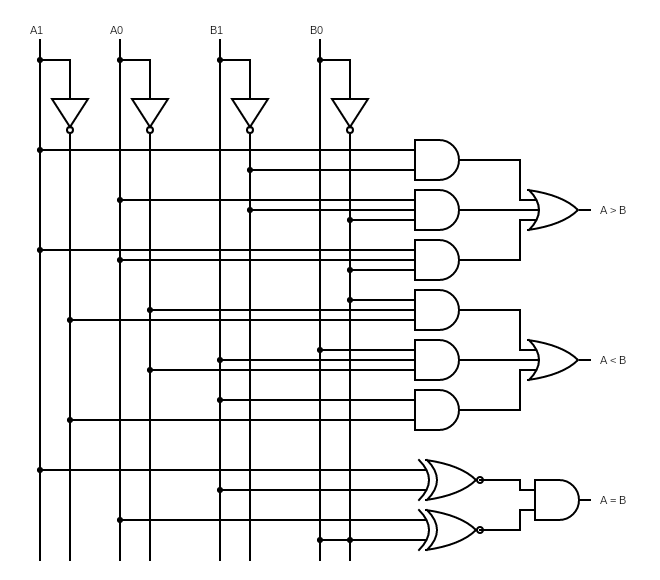
\includegraphics[height=10cm, width = 8cm]{circuit.png}
\end{figure}
  
  
 \section{Conclusion}
 
 
 In this report, we've discussed what magnitude comparators are, their applications, Boolean expressions for output, and implementation in FPGA.
  
\end{document}

